\documentclass[10pt,letterpaper]{article}
\usepackage[margin=1in]{geometry}
\usepackage[T1]{fontenc}
\usepackage{lmodern,microtype,amsmath,amssymb,amsthm,booktabs,array,graphicx,xurl}
\usepackage[hidelinks]{hyperref}
\usepackage{enumitem}
\microtypesetup{protrusion=false}
\setlist{nosep,leftmargin=*}
\setlength{\parskip}{3pt}
\setlength{\parindent}{1em}
\newtheorem{theorem}{Theorem}
\newtheorem{lemma}[theorem]{Lemma}
\newtheorem{proposition}[theorem]{Proposition}
\newtheorem{corollary}[theorem]{Corollary}
\newcommand{\ind}{\mathbf 1}
\newcommand{\R}{\mathbb R}
\newcommand{\dist}{\operatorname{dist}}
\newcommand{\D}{\mathcal D}
\newcommand{\F}{\mathcal F}
\title{Certified Expression Intervals under Shared Segmentation Uncertainty}
\author{Arnav Peram}
\date{}
\begin{document}
\hypersetup{pdftitle={Certified Expression Intervals under Shared Segmentation Uncertainty},pdfauthor={Arnav Peram},pageanchor=false}
\begin{titlepage}\maketitle\thispagestyle{empty}
\begin{abstract}\normalsize
A segmentation change can alter several transcript assignments through one shared boundary. We compute the observed cell-by-gene counts attainable under a specified physical deformation budget. For ordered boundaries with slope, band, thickness and nuclear constraints, one polynomial-size cut graph represents the minimum continuous deformation realizing every feasible assignment vector. We then construct disjoint two-label ribbons whose local maps glue into a topology-preserving deformation of the reference partition, with junction neighborhoods and uncovered boundary portions fixed. For scalar patches with explicitly represented point transcripts, an exact critical-height mesh and count-indexed shortest path compute every hard-budget count minimum in polynomial time, including outcomes missed by penalty optimization. Min-plus composition allocates one shared physical-area budget across compatible patches. Fixed geometric rules produce 544 patches on two public Xenium lung crops and 1,708 on two external breast format-test crops. Separate implementations agree on all 210,240 budgeted intervals. Among questions whose marginal interval reaches width at least two, exact geometry tightens 4 of 46 lung and 203 of 1,026 breast questions at some tested budget; 139 of 467 breast reference cells have an affected gene. Most endpoints still match the simple enclosure. The default family permits at most 0.451 micrometres of boundary displacement, and alternative segmentation counts often lie outside it. Rebuilt lung atlases with wider displacement caps still reach few changed nuclear-expansion or Proseg counts. The result is an exact compatible sensitivity calculation for retained counts under a declared fixed-seam family; anatomical calibration and biological accuracy remain open.
\end{abstract}
\thispagestyle{empty}\end{titlepage}
\hypersetup{pageanchor=true}\setcounter{page}{1}

\section{Introduction}
Imaging-based spatial transcriptomics turns detected molecules into a cell-by-gene matrix through a segmentation. An analyst interpreting a count needs to know whether a plausible change to the segmentation could alter it. Several molecules may move together, use the same physical deformation, or require incompatible boundaries. Independent molecule scores omit these dependencies, and separate local analyses require compatibility before they describe one partition.

We study a deterministic measurement question: for a fixed reference segmentation and an explicit deformation family, what are the smallest and largest retained counts attainable within an area budget? An answer contains a count interval, its geometric assumptions, and attaining boundaries. A singleton interval certifies invariance within that family. A wider interval identifies ambiguity in the observed count; anatomical correctness requires additional evidence.

Two obstacles are central. First, continuous boundary coordinates must be eliminated without losing the cost of jointly realizing molecular assignments. Second, local answers must compose into one partition and spend one shared budget. We address both constructively. The first result represents the entire assignment-cost function $D^\star(c)$ before objectives are chosen. The second supplies explicit homeomorphisms on disjoint ribbons, preserving the reference partition's topology. A count-indexed critical-height chain then gives exact hard-budget spectra for point transcripts on scalar patches, avoiding exponential assignment enumeration in that class.

\paragraph{Relationship to existing methods.}
Baysor, Proseg, BIDCell and Segger estimate segmentation or transcript assignments~\cite{baysor,proseg,bidcell,segger}. ResolVI models downstream misassignment probabilistically~\cite{resolvi}; ovrlpy examines three-dimensional signal overlap~\cite{ovrlpy}. TISSUE constructs uncertainty intervals for predicted, unmeasured expression~\cite{tissue}. Our intervals instead range over geometric alternatives for already observed molecules. They complement these estimators: a different estimated count supplies an alternative whose attainability can be tested.

Convex segmentation and ordered-label cuts~\cite{hochbaum,ishikawa}, interacting-surface graphs~\cite{li,shah}, higher-order energy constructions~\cite{kz,kohli}, Lipschitz extensions~\cite{petrakis}, and difference-potential lattices~\cite{felsner} provide foundations. Submodularity alone is insufficient for a binary graph representation with auxiliary variables~\cite{zivny}. We prove the particular cost-preserving elimination below. Exact critical heights offer another realization of that reduction; count augmentation uses established resource-state dynamic programming~\cite{hassin}. The advance to assess is the continuous assignment-cost identity and its compatible hard-budget realization, rather than the invention of cuts, shortest paths, or min-plus convolution.



\section{Continuous realization of assignments}\label{sec:continuous}
Use coordinate $t$ along an interface and $x$ across it. Let $m$ ordered boundary graphs $f_a:I\to\R$, $a=0,\ldots,m-1$, divide a compact corridor into $m+1$ cells. Each boundary has a constant slope limit $s_a>0$, a constant band $[\underline b_a,\overline b_a]$, and fixed endpoint values. Adjacent boundaries satisfy
\begin{equation}
0<d_a^{\min}\le f_{a+1}(t)-f_a(t)\le d_a^{\max}.\label{eq:gaps}
\end{equation}
The upper bound may be absent. A rational piecewise-affine reference $f^0$ satisfies these geometric constraints. Exterior rails strictly beyond the bands close the outer cells.

Site $i$ is a rectangle $[x_i^-,x_i^+]\times I_i$ in group $g(i)$; a point is a zero-size rectangle. All sites in a group share cell label $c_g$. Threshold bits $b_{ga}=\ind[c_g\le a]$ satisfy $b_{ga}\le b_{g,a+1}$. For clearance $\rho>0$, requiring the entire site to lie on its assigned side gives
\begin{equation}
 b_{g(i),a}=1\Rightarrow f_a(t)\ge \ell_i=x_i^++\rho,\qquad
 b_{g(i),a}=0\Rightarrow f_a(t)\le u_i=x_i^--\rho\quad(t\in I_i).\label{eq:owners}
\end{equation}
Fixed structural regions have pinned labels and no molecular reward. Nominal RNA locations use point sites. Universal-location regions use~\eqref{eq:owners}; they can make the source assignment inadmissible even though $f^0$ satisfies the geometry.

For a complete assignment $c$, let $\F(c)$ contain its realizing boundaries and define
\begin{equation}
D^\star(c)=\min_{f\in\F(c)}\sum_a\int_I |f_a(t)-f_a^0(t)|\,dt,
\qquad \min\varnothing=+\infty.\label{eq:dstar}
\end{equation}
This is summed interface displacement in the declared coordinates. The later scalar-ribbon construction converts it exactly to physical changed-label area counted once. For arbitrary unary molecular costs $C_g(c_g)$ and $\lambda\ge0$, the penalized objective is $\lambda D^\star(c)+\sum_g C_g(c_g)$; a hard area budget is a different problem.

\subsection{Propagation and exact feasibility}
Give the boundary-index graph an edge $a\to a+1$ of weight $d_a^{\min}$ and, when finite, a reverse edge of weight $-d_a^{\max}$. Let $\Delta_{ab}$ be maximum path weight, with $\Delta_{aa}=0$ and $-\infty$ for no path. Source feasibility excludes positive cycles. Define
\begin{equation}
K_{ab}(r)=\max_v\{\Delta_{av}+\Delta_{vb}-s_v r\},\qquad r\ge0.\label{eq:kernel}
\end{equation}
\begin{lemma}[Heterogeneous propagation]\label{lem:kernel}
Every feasible family obeys $f_b(y)\ge f_a(x)+K_{ab}(|x-y|)$. This is the strongest inequality obtained by finite compositions of the stated slope and same-coordinate difference constraints.
\end{lemma}
\begin{proof}
For any intermediate boundary $v$, transfer from $a$ to $v$ at $x$, travel on $v$ to $y$, and transfer to $b$. This gives each term of~\eqref{eq:kernel}. Conversely choose a boundary of smallest slope rate among the longitudinal portions of a composite path. Its vertical portions before and after that visit are bounded by $\Delta_{av},\Delta_{vb}$. Total absolute longitudinal travel is at least $|x-y|$, at rates at least $s_v$. Hence the path cannot improve that term. The zero-distance case follows from transitive closure.
\end{proof}
The kernels are nonincreasing, $K_{ab}(0)=\Delta_{ab}$, and $K_{ab}(r_1+r_2)\ge K_{av}(r_1)+K_{vb}(r_2)$. A term with rate greater than the destination rate $s_b$ is dominated by its direct-$b$ term; the analogous source statement holds.

A lower requirement $(a,I_i,\ell_i)$ is forbidden if a kernel term $(d,s)$ to any $b$ satisfies $\ell_i+d>\overline b_b$, or $\ell_i+d>f_b^0(e)+s\dist(e,I_i)$ at either endpoint $e$. An upper requirement $(a,I_i,u_i)$ is forbidden if a term of $K_{ba}$ satisfies $u_i-d<\underline b_b$, or $f_b^0(e)>u_i-d+s\dist(e,I_i)$. Add nesting and all fixed-label bits. Finally add
\begin{equation}
b_{g(i),a}\Rightarrow b_{g(j),b}
\quad\text{whenever }\ell_i+K_{ab}(\dist(I_i,I_j))>u_j.\label{eq:imp}
\end{equation}
These are finite unary restrictions and implications; a contradiction means an empty geometric family.

\begin{samepage}
\begin{theorem}[Feasible assignments]\label{thm:feas}
The finite restrictions characterize exactly the complete assignments realizable by the continuous family.
\end{theorem}
\end{samepage}
\begin{proof}
Necessity follows from Lemma~\ref{lem:kernel}; minimum interval distance gives the largest propagated lower requirement. For sufficiency, propagate all active lower requirements, bands and fixed endpoint values into $L_b(t)$, and upper requirements into $U_b(t)$. A lower term is $\ell_i+K_{ab}(\dist(t,I_i))$; an upper term from $a$ is $u_i-K_{ba}(\dist(t,I_i))$. Kernel composition, the triangle inequality, and~\eqref{eq:imp} put every lower term below every upper term. Unary restrictions handle fixed data, so $L_b\le U_b$.
For a directed gap edge $a\to b$ of weight $d$, closure gives $K_{vb}\ge K_{va}+d$ and $K_{av}\ge d+K_{bv}$. Thus $L_b\ge L_a+d$ and $U_a\le U_b-d$. Applying this to reverse edges enforces maximum gaps as well. Dominated rates preserve individual slope limits. Fixed data enforce bands and endpoint equality. Both envelope families therefore satisfy the geometry and realize the selected requirements. Nesting decodes one label per group.
\end{proof}

\subsection{An exact cost function before molecular objectives}
\begin{samepage}
\begin{theorem}[Assignment-wise cost representation]\label{thm:cost}
For rational input, a polynomial-size directed graph with assignment bits $b(c)$, helpers $y$, rational capacities, hard implications and known constant $\kappa$ satisfies
\begin{equation}
\min_y\operatorname{Cut}_{G_D}(b(c),y)+\kappa=D^\star(c)\label{eq:identity}
\end{equation}
for every feasible $c$. Hard-feasible cuts exist exactly for feasible assignments. For arbitrary rational unary molecular costs and rational $\lambda\ge0$, a cut either detects infeasibility or returns an optimum and an attaining rational piecewise-affine boundary.
\end{theorem}
\end{samepage}
\begin{proof}
The family of lower difference inequalities is closed under componentwise minimum and maximum; those operations also preserve each scalar slope bound, band and endpoint. Since $L,U,f^0$ obey the geometry,
\begin{equation}
f_b^*(t)=\min\{U_b(t),\max\{L_b(t),f_b^0(t)\}\}\label{eq:clamp}
\end{equation}
is jointly feasible and satisfies the selected requirements. Every realization has $L_b(t)\le f_b(t)\le U_b(t)$. The clamp is the nearest permitted value to $f_b^0(t)$ at every coordinate, proving simultaneous minimum displacement and~\eqref{eq:dstar}.

An upward displacement is the maximum of nonnegative functions $[\ell_i+d-s\dist(t,I_i)-f_b^0(t)]_+$ activated by bits; downward displacements use complementary bits. Include structural requirements and source-inconsistent RNA requirements. Upward and downward contributions cannot both be positive on a feasible assignment. Split the domain at their affine-piece endpoints, zeros, source knots and pair crossings. On one slab let $h_1\ge\cdots\ge h_k>0$, $h_{k+1}=0$, with $S_j$ the labels in the first $j$ activations. Then
\begin{equation}
\max_{i\text{ active}}h_i=\sum_{j=1}^k(h_j-h_{j+1})\ind[S_j\text{ contains an active bit}].\label{eq:layers}
\end{equation}
Integrate the nonnegative affine differences exactly. An OR term has a standard helper with incoming hard implications and a terminal cost; complementary terms reverse the construction~\cite{kz,kohli}. Repeated labels are included once. Fixed terms are retained in $\kappa$ or forced helpers. Thus minimizing over helpers gives the exact integrated clamp for each fixed $b(c)$, proving~\eqref{eq:identity}. Expand any unary cost as $C_g(m)+\sum_{a<m}[C_g(a)-C_g(a+1)]b_{ga}$ and shift negative terms by a known constant. Rational scaling yields integer capacities. The topology and geometric coefficients are fixed before molecular costs; numerical hard capacities are instantiated above the total finite capacity after the costs and $\lambda$ are chosen. This distinguishes infeasibility;~\eqref{eq:clamp} reconstructs the boundary.
\end{proof}

\paragraph{Graph size versus construction work.}
Let $N$ count all merged RNA and structural rectangles, $G$ groups, and $M_b=O(Nm^2)$ propagated terms on boundary $b$. For one polarity the untruncated terms are $g_i(t)=\alpha_i-s_i\dist(t,I_i)$. Their common reference changes positivity while preserving relative cone order. Each pair changes order only constantly many times. An adjacent swap changes one full prefix; starting with $M_b$ prefixes yields $O(M_b^2+M_b)$ distinct activation sets. Simultaneous events may be resolved into adjacent swaps, repeated labels only merge sets, and zero-weight predecessor prefixes support constant-arc helpers. Consequently
\begin{equation}
|V|=O\!\left(Gm+\sum_b(M_b^2+M_b)\right),\quad
|E|=O\!\left(Gm+N^2m^2+\sum_b(M_b^2+M_b)\right).\label{eq:size}
\end{equation}
The auxiliary contribution is $O(N^2m^5)$. Source knots still affect integration, coefficient lengths and reconstruction. Exact intersections, integrals and denominator scaling have polynomial bit complexity. An event sweep integrates the coefficients exactly; its construction bound and operand-cost qualifications are given in the supplement. Arrangement sweeps are established tools~\cite{bentley}.

\section{From local interfaces to one compatible tissue model}\label{sec:atlas}
Applying separate corridors to the same RNA can produce different intervals because the corridors are different models. We instead specify one \emph{atlas}: disjoint two-label ribbons around selected reference interfaces, with fixed endpoint traces and outer rails. The rest of the partition stays fixed. A single atlas identity is attached to all its cell-count outputs.

Let $P_i$ be closed ribbons with pairwise disjoint interiors and injective charts $\Psi_i:I_i\times[-B_i,B_i]\to P_i$. The reference boundary is transverse coordinate zero, each half lies wholly in its stated reference label, and each RNA belongs to at most one ribbon. An allowed displacement $h_i$ is continuous, zero at both endpoints, and $|h_i|\le qB_i$ for $q<1$. Fixed regions have additional label constraints.

\begin{samepage}
\begin{theorem}[Compatible gluing and additive physical area]\label{thm:glue}
Every tuple of admissible ribbon boundaries is induced by one global homeomorphism of the reference partition, identity outside the ribbon interiors. For constant chart Jacobians $J_i>0$, the physical area whose label changes is exactly $\sum_i J_i\int|h_i|$.
\end{theorem}
\end{samepage}
\begin{proof}
For fixed $t$, define a map of $[-B_i,B_i]$ by
\begin{equation}
H_i(t,v)=\begin{cases}
-B_i+(v+B_i)(h_i(t)+B_i)/B_i,&v\le0,\\
h_i(t)+v(B_i-h_i(t))/B_i,&v\ge0.
\end{cases}\label{eq:homeo}
\end{equation}
The two positive slopes are bounded away from zero; both branches meet at $h_i(t)$ and have continuous explicit inverses. The map fixes rails and is identity at the interval endpoints. Conjugating $(t,v)\mapsto(t,H_i(t,v))$ by $\Psi_i$ gives a homeomorphism fixing the entire ribbon boundary. Extend by identity outside. Finitely many such maps and inverses agree on intersections, so they glue continuously and bijectively. Cell topology and fixed junction incidences are preserved. The changed-label region in one ribbon lies between zero and $h_i(t)$, with chart area $\int|h_i|$. Change of variables and disjoint interiors give the sum.
\end{proof}

\paragraph{Exact chart for a raster interface.}
For a coordinate-monotone raster-edge path choose $s_x,s_y\in\{-1,1\}$ and let $t=s_xx+s_yy$, $u=s_xx-s_yy$ in pixel coordinates. The exact source arc is $u=r_i(t)$. With pixel size $p$,
\begin{equation}
\Psi_i(t,h)=\frac p2\big(s_x(t+r_i(t)+h),\ s_y(t-r_i(t)-h)\big),\qquad J_i=p^2/2,\label{eq:chart}
\end{equation}
up to the recorded origin. This piecewise-affine shear preserves the original staircase interface exactly. Its Jacobian is constant even at changes of source slope, apart from measure-zero corners. The local optimization variable is displacement $h$, with zero source; source corners are chart-slope changes rather than new topological junctions. Intersecting nuclear pixels induce conservative exact interval constraints in this chart. Their labels are preserved; their material motion is unspecified.

\paragraph{Theorem--application alignment.}
Every evaluated atlas ribbon has one moving interface. Its solver uses the scalar specialization of Section~\ref{sec:continuous}, the critical-mesh count algorithm and compatible composition. The coupled multi-boundary propagation theorem describes a broader exact class; its thickness coupling is not exercised by the atlas experiment.

This family can follow arbitrary reference adjacency because junction neighborhoods remain fixed. Topology and uncovered perimeters stay fixed. Coverage is therefore part of the model definition.

\begin{figure}[t]\centering
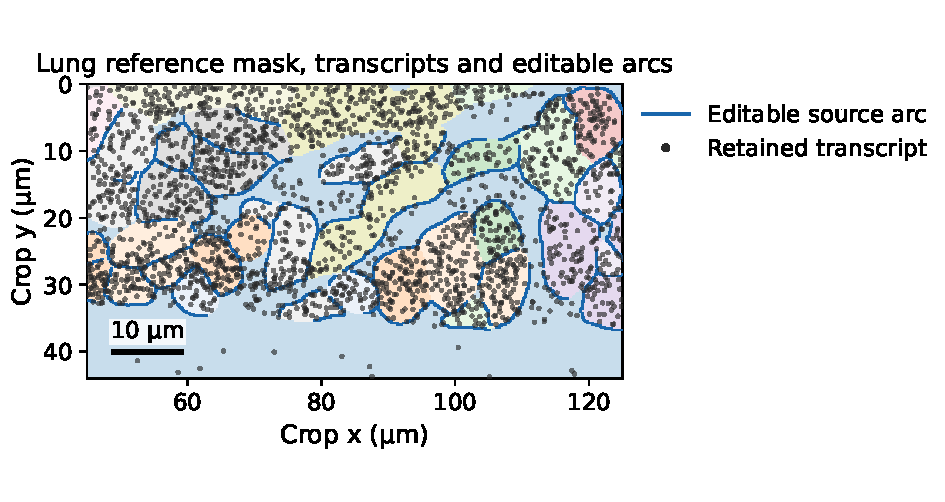
\includegraphics[width=.90\textwidth]{figures/atlas_reference.pdf}
\caption{Actual reference labels and retained transcript positions in a lung-crop excerpt; blue lines mark the source arcs of accepted disjoint ribbons. Scale bar: $10\,\mu\mathrm m$. Shared-boundary arcs remain part of the original raster partition. Endpoint seams, junction neighborhoods and uncovered portions are fixed. Every edited ribbon maps into the same global partition rather than defining another overlapping local model.}\label{fig:atlas}
\end{figure}

\section{Hard budgets without an assignment enumeration}\label{sec:counts}
For a retained count $N_{kg}(c)$, define the minimum-area spectrum
\begin{equation}
S_{kg}(q)=\min_{c:N_{kg}(c)=q}D^\star(c),\quad
[L_{kg}(\delta),U_{kg}(\delta)]=\left[\min,\max\right]\{q:S_{kg}(q)\le\delta\}.\label{eq:interval}
\end{equation}
The notation means the smallest and largest elements of the displayed feasible-count set. Its interior need not contain every integer. A witness for each endpoint proves attainment; an empty set is reported separately.

\subsection{Exact critical heights and a count chain}
For one boundary, collect all propagated lower/upper requirement pieces, fixed geometric pieces and source pieces before selecting owners. A common mesh contains all piece endpoints and crossings, including source crossings and every point observation. At node $t_j$, retain their candidate values $V_j$ within forced envelopes and discard values violating any point's clearance gap or fixed constraint.

\begin{lemma}[Exact scalar critical mesh]\label{lem:mesh}
Restricting nodal heights to these candidates, enforcing original adjacent slope and ownership constraints, and charging trapezoidal absolute displacement preserves $D^\star(c)$ for every feasible assignment.
\end{lemma}
\begin{proof}
Between consecutive events all candidate pieces are affine and their ordering is fixed. The canonical clamp~\eqref{eq:clamp} selects one such piece and has constant-sign displacement. Its nodal candidates are retained and its trapezoidal area equals its exact integral. Conversely a feasible candidate-height path interpolates to a feasible continuous boundary: every constraint endpoint is in the mesh, and the intervening constraints are linear. The trapezoid upper-bounds that interpolant's absolute-displacement integral, which is at least $D^\star(c)$. The retained canonical minimizer attains equality.
\end{proof}

\begin{samepage}
\begin{theorem}[Polynomial exact spectra for explicit point RNAs]\label{thm:chain}
Assume one boundary, one point per free RNA group, arbitrary fixed structural intervals, and a nonnegative integer per-point count score. Let $W$ be its variable range and $H_j=|V_j|$. Given the critical mesh and its local node scores, the count dynamic program uses $O((W+1)\sum_jH_j)$ arithmetic transition operations and returns every minimum-area count, with backpointers to attaining boundaries. With explicit unit transcripts the complete algorithm is polynomial in the input and rational encoding.
\end{theorem}
\end{samepage}
\begin{proof}
A permitted height at a point's mesh node uniquely determines its owner, since the clearance gap was excluded. Count each observation once at that node. Let $z_j(h)$ be its local score and $a_j(h)=w_j|h-f^0(t_j)|$, where $w_j$ is half the sum of adjacent mesh lengths. Define
\begin{equation}
F_j(h,q)=a_j(h)+\min_{u\in V_{j-1}:|u-h|\le s(t_j-t_{j-1})}
F_{j-1}(u,q-z_j(h)).\label{eq:dp}
\end{equation}
Initialization accounts for fixed groups and the first node. The shortest-path induction gives the exact nodal minimum for every count. Lemma~\ref{lem:mesh} gives continuous equality, including unsupported penalty outcomes. For each predecessor count, allowed sorted predecessors form a sliding interval as $h$ increases. A monotone queue computes its minima in $O(H_{j-1}+H_j)$ operations. Sum over counts and nodes. Backpointers reconstruct candidates and hence attaining boundaries.
If $P$ is the total affine-piece count, a full mesh has $O(P^2+P)$ nodes and $O(P)$ candidates per node; this and rational intersection arithmetic give polynomial preparation and encoding. For unit RNA scores, $W$ is bounded by the explicit molecule count. Binary-compressed multiplicities instead give a pseudo-polynomial count dependence. Free interval-valued RNA groups and arbitrary coupled height vectors require additional state and are outside this scalar result.
\end{proof}

Resource-state shortest paths are standard~\cite{hassin}. Here the critical-mesh proof supplies exact continuous costs for each resource state, rather than treating a user-chosen mesh as exact. Single-copy queries use a cheaper corollary: when the source satisfies every source-owner and structural constraint at zero cost, propagate requested bits, keep unforced source bits, and reconstruct the clamp. Every costly requirement in that completion is forced in all feasible completions, so it is minimum-area. The count-chain theorem applies without this stronger source-assignment premise.

\subsection{One area allowance for the entire atlas}
For a fixed cell and gene, compute each incident patch's spectrum $S_i(d)$ in \emph{count changes} relative to its source. Let $n^0_{kg}$ include all retained RNA in that reference cell, including outside the ribbons. Then
\begin{equation}
S_{kg}(q)=\min_{d_1+\cdots+d_r=q-n^0_{kg}}\sum_{i=1}^r S_i(d_i).\label{eq:convolution}
\end{equation}
This is min-plus convolution. An attaining trace selects one witness per patch, and Theorem~\ref{thm:glue} gives a valid global partition. Conversely every allowed partition decomposes into patch states costing at least their local minima. These two directions prove~\eqref{eq:convolution}. Patches with no relevant gene can stay at their zero-cost source. A simple convolution takes $O(rW^2)$ operations. Thus scalar point-RNA patch atlases give polynomial exact single-cell/gene spectra despite arbitrary fixed reference adjacency.

No molecule or exterior count is duplicated, and $\delta$ is spent once. Every allowed full count matrix lies componentwise inside the table, but different rows' endpoints need not coexist. Joint marker questions require vector spectra or a joint predicate query, rather than multiplying marginal endpoint sets.

\subsection{Why a penalty path alone is insufficient}
An exact cut yielding $m(\mu)=\min_{c:\F(c)\ne\varnothing}\{\mu D^\star(c)-N(c)\}$ gives
\begin{equation}
U(\delta)\le\left\lfloor\mu\delta-m(\mu)\right\rfloor,\qquad\mu\ge0.\label{eq:dual}
\end{equation}
This is weak duality. Feasible witnesses give the opposite bound; a gap is retained unless exact refinement closes it. Applying the same argument to $-N$ bounds the lower endpoint.

A gap occurs even with eight \emph{distinct, explicit unit} transcripts. Take source zero on $[0,30]$, slope one, band $[-4,4]$, and clearance $1/10$. At longitudinal centers $5,15,25$, place clusters of $2,3,3$ RNAs. In a cluster of height $a=2,3,3$, respectively, point $j$ is $(t,x)=(\mathrm{center}+j/100,a-j/100-1/10)$. Clearance forces common ownership within each cluster; its first cone dominates, and cluster supports are disjoint. The exact count/area states are $(0,0),(2,4),(3,9),(5,13),(6,18),(8,22)$. At budget ten the maximum is three, whereas the best penalty upper bound is four: for $\mu\le1/3$, the count-eight state gives $B(\mu)\ge8-12\mu\ge4$; for $\mu\ge1/3$, the count-two state gives $B(\mu)\ge2+6\mu\ge4$. Equality holds at $1/3$. The count chain recovers the unsupported count-three state. The example uses no binary-encoded multiplicity.

\section{Evaluation on one development dataset and external test data}\label{sec:eval}
\subsection{Fixed-rule construction and physical coverage}
Two existing lung crops contain 7,370 retained Q20 measured-gene records~\cite{data,xenium}. Reference labels come directly from masks. Eligibility requires a source cell to be connected and avoid crop borders. All interfaces between eligible cells or an eligible cell and background are considered. Geometry-only rules trace monotone arcs, cap runs at 128 edges, freeze one edge at each end, retain at least four edges, and try ribbon halfwidths $4,2,1,1/2$ pixels. Longer arcs are processed first with deterministic coordinate ties. Exact rational intersection checks certify half-ribbon labels and disjoint interiors. The displacement band is $3B/4$, slope limit one, and chart clearance $10^{-6}/p$ pixels. Nuclear fragments become pinned interval requirements. Widths, selection, slope and budgets are declared sensitivity settings. All four source transforms give $p=1048576/4934475\simeq0.212500013\,\mu\mathrm m$ per pixel. Equation~\eqref{eq:chart} converts transverse displacement to Euclidean distance $p|h|/\sqrt2$. Thus $B\le4$ and $|h|\le3B/4$ imply a physical bound of $0.450781\,\mu\mathrm m$ before further slope or nuclear restrictions.

The complete atlas, rather than a set of overlapping windows, is the input to every count question. Our initial nucleus-free extraction was amended to retain pinned nuclear constraints and cell--background interfaces before count outcomes were computed. That developmental amendment is recorded. The same rules were then applied without retuning to two previously acquired breast crops containing 81,182 retained RNAs. The breast source is the vendor's trimmed two-FOV \emph{format-test} dataset, explicitly unsuitable for biological conclusions~\cite{breasttest}. Its role is external computational transfer testing; it supplies neither ownership truth nor held-out biological validation.

\begin{table}[t]\centering
\begin{tabular}{lrr}\toprule
Quantity & Lung & Breast format test\\\midrule
Crop-contained connected reference cells &153&467\\
Accepted disjoint patches &544&1,708\\
All retained RNA records &7,370&81,182\\
RNA inside editable ribbons &745&8,262\\
Editable / all incident boundary edges &15,821 / 23,164&52,912 / 80,463\\
Coverage of all incident reference edges &68.3\%&65.8\%\\
Positive-or-editable cell--gene entries &3,304&22,976\\
Exact intervals at eight budgets &26,432&183,808\\\bottomrule
\end{tabular}
\caption{All eligible reference cells remain, including cells with no editable boundary. Cells and repeated budgets are correlated measurement objects. The denominator includes incident boundaries excluded because the neighbor intersects the crop border. Uncovered interfaces and seams stay fixed.}\label{tab:scope}
\end{table}

\subsection{Exact counts, simple bounds and shared-budget effects}
Budgets are $0,0.05,0.1,0.25,0.5,1,2,4\,\mu\mathrm m^2$. We retain every positive-or-editable cell--gene entry, with omitted zero entries specified by a matrix index. One atlas, source count and cell identifier define each row uniquely. A separate scalar integration and Cartesian-composition implementation confirms all 210,240 intervals. The polynomial count chain additionally matches all 944 multi-copy patch/gene spectra; single-copy queries use closure. Complete hybrid re-execution reproduces the same cell spectra.

The strong marginal outer bound allows every transcript whose individual transfer cost is at most $\delta$ to move simultaneously. It can violate the shared budget or combine incompatible moves. A separate additive \emph{inner} approximation retains exact joint feasibility but replaces shared area by summed singleton minima for every changed transcript, including collateral genes. Under source admissibility, shared maximum-envelope area is at most that sum. Thus its count range is contained in the exact range, which is contained in the marginal outer range.

\begin{table}[t]\centering
\begin{tabular}{lrr}\toprule
Complete eight-budget census & Lung & Breast test\\\midrule
Rows tighter than marginal outer bound &4 / 26,432&228 / 183,808\\
Rows with endpoints missed by additive inner model &2 / 26,432&68 / 183,808\\
Non-singleton intervals at $\delta=0.1$ &429 / 3,304&4,414 / 22,976\\
Non-singleton intervals at each $\delta\in\{0.25,0.5,1,2,4\}$ &524 / 3,304&5,259 / 22,976\\
Questions tightened / marginal width $\ge2$ &4 / 46&203 / 1,026\\
Largest count width over all budgets &3&10\\\bottomrule
\end{tabular}
\caption{Most answers coincide with simpler reasoning. The outer and inner comparisons isolate different approximation losses.}\label{tab:counts}
\end{table}

The question-level denominator is defined without selecting successful outputs: a cell--gene question qualifies when its marginal interval has width at least two at any tested budget. The numerator counts each qualifying question once if exact geometry tightens any tested interval. The fractions are 4/46 (8.7\%) in lung and 203/1,026 (19.8\%) in breast; the latter involve 139/467 reference cells (29.8\%). Whole-census row totals remain in Table~\ref{tab:counts}. These are descriptive counts on correlated queries.

Constant non-singleton totals do not establish endpoint saturation. In breast, 61 questions change an endpoint between budgets 0.25 and 0.5, and three more between 0.5 and 1. Lung endpoints plateau on the sampled grid from 0.25; breast endpoints plateau from 1. All marginal improvements occur at budgets at most 0.5. Both limited displacement reach and the concentration of budget effects at small areas must inform interpretation.

In an illustrative breast-test reference cell, the retained LDHB source count is 22. At $0.25\,\mu\mathrm m^2$, its exact interval is $[19,23]$, while the marginal outer interval is $[17,23]$: individually affordable changes cannot all share that budget. At $0.5\,\mu\mathrm m^2$, the exact interval is $[17,23]$, while the additive inner model gives $[18,23]$. The attaining lower witness moves three LDHB transcripts through one boundary patch and two through another, together with one collateral KRT8 transcript. Their physical areas are approximately $0.342327$ and $0.141713\,\mu\mathrm m^2$, totaling $0.484040$. This example was selected after the complete census for illustration; its interpretation is confined to this count model.

\begin{figure}[t]\centering
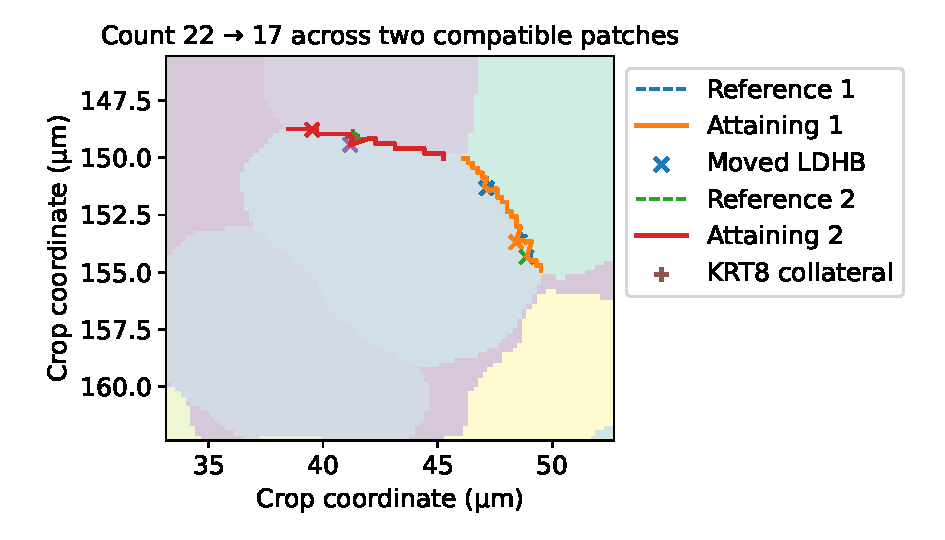
\includegraphics[width=.90\textwidth]{figures/cell_witness.pdf}
\caption{Actual source-mask geometry and an attaining two-patch witness in the external format-test crop. Cross markers identify the five LDHB molecules leaving reference cell 81; a plus marker identifies collateral KRT8. Both patch changes belong to the same globally glued family. The example illustrates attainable counts and shared-budget accounting.}\label{fig:witness}
\end{figure}



\subsection{Co-detection and an alternative image-only reference}
The supplementary co-detection census retains all EPCAM/PTPRC, EPCAM/CD3D and EPCAM/PECAM1 questions. None adds an exclusion beyond its marginal bounds; these predicates remain model-conditioned detection statements.

A distinct image-only reference assigns each pixel to its nearest labelled nuclear pixel within $5\,\mu\mathrm m$, and to background otherwise. Nuclear labels are read from the source cell mask. We exclude transcripts within $5\,\mu\mathrm m$ of the crop boundary and exclude a gene if that exclusion intersects an editable part of its spectrum. No atlas parameter is changed. Under this original protocol, 1,818 of 11,151 changed breast-test counts are attainable anywhere in the atlas. The following lung width study uses a refined shared-population contract documented in the supplement. Full retained alternative assignment vectors are infeasible in all four crops, including many changes outside editable ribbons. This directly exposes the family's limited reach. Entrywise reach is a model diagnostic, rather than accuracy against truth or joint feasibility of the alternative matrix. The following comparison additionally uses actual Proseg outputs.

\subsection{Physical reach and an executed segmentation comparison}
Proseg 3.2.0 completed on both lung crops after disabling factorization following a default-run failure on the first small crop. It retained 5,774 and 1,482 transcripts, excluding 73 and 41. We compare counts on shared retained IDs at the original observed coordinates; Proseg's diffused coordinates define a different observation problem. These same-donor, sparse-crop runs provide alternative counts, rather than ownership truth.

A post-review protocol fixed three width settings before rerunning geometry-only extraction. The largest band-implied displacement caps among accepted patches are $0.451$, $1.352$ and $3.155\,\mu\mathrm m$. The enlarged halfwidth is accepted in 132 of 544 intermediate-cap patches and 41 of 543 largest-cap patches; the others retain halfwidth at most 4. At unlimited area, reachable changed nuclear counts are $186/1{,}134$, $223/1{,}134$ and $190/1{,}134$; Proseg counts are $185/2{,}798$, $241/2{,}798$ and $200/2{,}798$ (Fig.~\ref{fig:reach}). Exact score-spectrum membership is tested, including gaps between attainable counts. Excluded molecules remain zero-score geometric constraints. This refines the original nuclear protocol by retaining six additional boundary-gene questions, one reachable. Greedy reconstruction and different fallback ladders produce non-nested families, explaining why reach can decrease at the largest cap. Even the best tested setting reaches only $19.7\%$ of changed nuclear counts and $8.6\%$ of changed Proseg counts. Width and area increases therefore leave substantial restrictions from fixed seams, candidate neighbors and nuclear constraints.

\begin{figure}[ht]
\centering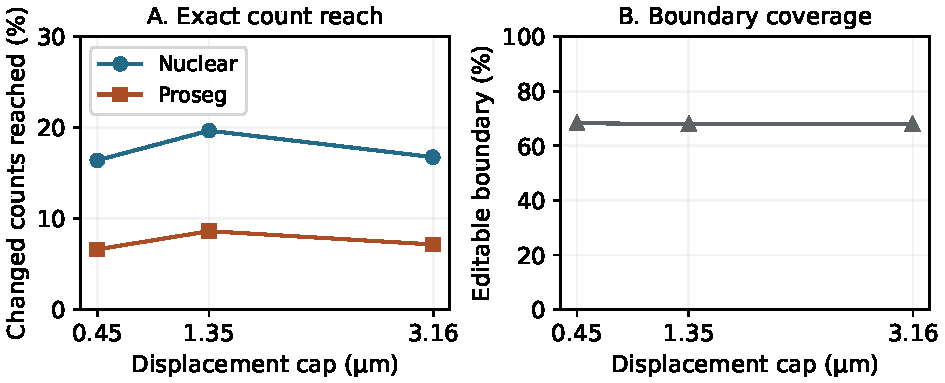
\includegraphics[width=.96\textwidth]{figures/reach_width.pdf}
\caption{Lung width sensitivity on fixed comparison populations. Left: exact countwise reach at unlimited area. Right: editable fraction of eligible-cell incident boundary edges. The rebuilt atlases are non-nested; connecting lines organize the tested settings. Reach describes each count separately, rather than joint feasibility or biological accuracy.}
\label{fig:reach}
\end{figure}


\subsection{Algorithmic checks and measured operating range}
The count chain agrees with 201 random scalar spectra, 80 additional nonflat models with exhaustive owners, a positive-mandatory-area case, and the eight-unit-RNA gap. Free horizontal or longitudinal location intervals, free multisite groups and overlapping ownership thresholds are rejected by its input contract. Loaded atlases are checked against source identity and completed geometric audits before certification. Source-coordinate checks verify every retained molecule's original label; rational pixel-overlap checks verify atlas geometry and nuclear coverage. A separate scalar implementation, which imports no production implication, envelope or cut routine, reconstructs 7,774 local spectra and checks their composed extrema against Cartesian enumeration. Prepared data extraction remains shared.

An analytically solvable family tests all count levels for 16, 32, 64 and 128 explicit RNAs. Median complete times over three fresh processes are 0.465, 1.574, 7.138 and 42.206 seconds. The largest run returns 129 levels with checked witnesses using 605,632 height/count states. The supplement records the analytical formula, stage times and limits.

\section{Discussion and reproducibility}
The mathematical result and application now share one object: an exact count-versus-area spectrum induced by compatible continuous partitions. The ownerwise reduction establishes cost preservation. Critical heights and an explicit count counter recover hard-budget outcomes, while disjoint support and fixed traces turn local realizations into a global one. Direct cut layers remain useful for arbitrary unary molecular objectives and sound Lagrangian bounds; the scalar count chain is a different algorithm for a stronger constrained output.

The atlas is a fixed-seam sensitivity model. It covers approximately two-thirds of incident reference boundary length on these crops, with the remaining geometry fixed. Its geometric settings are uncalibrated, the breast data are format tests, and reporter-labelled ownership truth and multi-donor biological evaluation remain unavailable. The adapted Proseg runs use the same sparse lung crops, so they test reach rather than ownership accuracy. Simple bounds explain most endpoints; a deterministic alternative segmentation often falls outside the family. These results limit anatomical interpretation rather than the conditional exactness of the computation. Differential-expression significance, false-discovery guarantees and ligand--receptor signaling require additional statistical assumptions and evidence beyond count intervals.

\paragraph{Code, data and assistance.}
Scientific code is frozen at revision \href{https://github.com/arnavperam/geocert/tree/1cdbb9e0b4ea386c210fd231372900b2844dddba/atlas2027}{\nolinkurl{1cdbb9e0b4ea386c210fd231372900b2844dddba}}. Source code, exact results, witnesses and reproduction commands are available at \url{https://github.com/arnavperam/geocert/tree/atlas-merged-revision/atlas2027}. Project software is MIT licensed. Data attribution follows the original 10x CC BY 4.0 terms. AI assistance contributed to mathematical development, algorithm design, code, experiments, checking and drafting. Authorship and responsibility for the content rest with the listed author. Computational checking uses separate implementations; human theorem review remains a distinct assessment.

\clearpage
\begin{thebibliography}{99}
\bibitem{baysor} V. Petukhov et al. Cell segmentation in imaging-based spatial transcriptomics. \emph{Nature Biotechnology} 40:345--354, 2022. doi:10.1038/s41587-021-01044-w.
\bibitem{proseg} D. C. Jones, A. E. Elz, A. Hadadianpour, H. Ryu, D. R. Glass, and E. W. Newell. Cell simulation as cell segmentation. \emph{Nature Methods} 22:1331--1342, 2025. doi:10.1038/s41592-025-02697-0.
\bibitem{li} K. Li, X. Wu, D. Z. Chen and M. Sonka. Optimal surface segmentation in volumetric images---a graph-theoretic approach. \emph{IEEE TPAMI} 28(1):119--134, 2006. doi:10.1109/TPAMI.2006.19.
\bibitem{shah} A. Shah, M. D. Abramoff and X. Wu. Optimal surface segmentation with convex priors in irregularly sampled space. \emph{Medical Image Analysis} 54:63--75, 2019. doi:10.1016/j.media.2019.02.004.
\bibitem{petrakis} I. Petrakis. McShane--Whitney extensions in constructive analysis. \emph{Logical Methods in Computer Science} 16(1):18, 2020. doi:10.23638/LMCS-16(1:18)2020.
\bibitem{kz} V. Kolmogorov and R. Zabih. What energy functions can be minimized via graph cuts? \emph{IEEE TPAMI} 26(2):147--159, 2004. doi:10.1109/TPAMI.2004.1262177.
\bibitem{data} 10x Genomics. Preview Data: FFPE Human Lung Cancer with Xenium Multimodal Cell Segmentation. 5 February 2024. One donor; CC BY 4.0. \url{https://www.10xgenomics.com/datasets/preview-data-ffpe-human-lung-cancer-with-xenium-multimodal-cell-segmentation-1-standard}.
\bibitem{xenium} 10x Genomics. Understanding Xenium Outputs: cell and nucleus segmentation files. Documentation accessed 26 October 2026. \url{https://www.10xgenomics.com/support/software/xenium-onboard-analysis/3.2/analysis/xoa-output-understanding-outputs}.
\bibitem{felsner} S. Felsner and K. Knauer. Distributive lattices, polyhedra, and generalized flows. \emph{European Journal of Combinatorics} 32(1):45--59, 2011. doi:10.1016/j.ejc.2010.07.011.
\bibitem{resolvi} C. Ergen and N. Yosef. ResolVI: addressing noise and bias in spatial transcriptomics. \emph{Nature Methods} 23:2003--2014, 2026. doi:10.1038/s41592-026-03212-9.

\bibitem{hochbaum} D. S. Hochbaum. An efficient algorithm for image segmentation, Markov random fields and related problems. \emph{Journal of the ACM} 48(4):686--701, 2001. doi:10.1145/502090.502093.
\bibitem{ishikawa} H. Ishikawa. Exact optimization for Markov random fields with convex priors. \emph{IEEE TPAMI} 25(10):1333--1336, 2003. doi:10.1109/TPAMI.2003.1233908.
\bibitem{kohli} P. Kohli, L. Ladick\'y and P. H. S. Torr. Robust higher order potentials for enforcing label consistency. \emph{International Journal of Computer Vision} 82:302--324, 2009. doi:10.1007/s11263-008-0202-0.
\bibitem{zivny} S. \v{Z}ivn\'y, D. A. Cohen and P. G. Jeavons. The expressive power of binary submodular functions. \emph{Discrete Applied Mathematics} 157(15):3347--3358, 2009. doi:10.1016/j.dam.2009.07.001.
\bibitem{bidcell} X. Fu et al. BIDCell: Biologically-informed self-supervised learning for segmentation of subcellular spatial transcriptomics data. \emph{Nature Communications} 15:509, 2024. doi:10.1038/s41467-023-44560-w.
\bibitem{segger} E. Heidari, A. Moorman et al. Segger: Fast and accurate cell segmentation of imaging-based spatial transcriptomics data. \emph{bioRxiv}, 2025. doi:10.1101/2025.03.14.643160.
\bibitem{ovrlpy} S. Tiesmeyer et al. Identifying 3D signal overlaps in spatial transcriptomics data with ovrlpy. \emph{Nature Biotechnology}, 2026. doi:10.1038/s41587-026-03004-8.

\bibitem{bentley} J. L. Bentley and T. A. Ottmann. Algorithms for reporting and counting geometric intersections. \emph{IEEE Transactions on Computers} C-28(9):643--647, 1979. doi:10.1109/TC.1979.1675432.

\bibitem{tissue} E. D. Sun, R. Ma, P. Navarro Negredo, A. Brunet and J. Zou. TISSUE: uncertainty-calibrated prediction of single-cell spatial transcriptomics improves downstream analyses. \emph{Nature Methods} 21:444--454, 2024. doi:10.1038/s41592-024-02184-y.
\bibitem{hassin} R. Hassin. Approximation schemes for the restricted shortest path problem. \emph{Mathematics of Operations Research} 17(1):36--42, 1992. doi:10.1287/moor.17.1.36.
\bibitem{breasttest} 10x Genomics. Example Xenium datasets, XOA 2.0: two-FOV human breast multimodal-segmentation format test. CC BY 4.0. \url{https://www.10xgenomics.com/support/software/xenium-onboard-analysis/2.0/resources/xenium-example-data}. Accessed 28 October 2026.
\end{thebibliography}
\end{document}
